
\chapter{Framework Verification \label{chap:08-Real-world_network_planning}}

% First paragraph has no indentation.

\noindent The objective of Chapter~\ref{chap:05-Framework_parameter_tuning}
was to ease the execution of radio-network planning activities, the
complexity of which is generally beyond the scope of a manual approach.
In this context, PRATO was presented as a tool that can help an engineer
in realizing his or her everyday network-planning tasks.

Another important factor to further validate the adoption of the presented
framework is to verify its accuracy. This is especially important
in real-world scenarios, where it is not feasible to improve the performance
of radio-coverage predictions at the cost of precision loss. The scope
of this chapter is therefore to establish that the accuracy of the
radio-propagation predictions of PRATO, as described previously in
Chapter~\ref{chap:04-Framework-design-and-implementation}, is adequate
for real-world, radio-network planning purposes. To this end, and
with the help of the radio engineers at Telekom Slovenije, d.d., some
real-world radio-propagation scenarios are calculated using PRATO
and an enterprise, industrial software. During the experimentation
phase, as well as when comparing the outcome, the engineers provided
guidelines to assess the results from a practical radio-network planning
perspective. The objective is to compare both tools in terms of solution
quality and computational-time performance. 

The rest of this chapter is organized as follows. Section~\ref{sec:08-Motivation}
gives an overview of the reasons behind the verification of the framework.
A description of the testing environment, including three networks,
is given in Section~\ref{sec:08-Radio_environment_setup}, followed
by an extensive performance analysis of the simulation results in
Section~\ref{sec:08-Performance_analysis}.


\section{Motivation \label{sec:08-Motivation}}

For a mobile operator, the utilization of a radio-network planning
tool has clear economical and technical benefits. As it has been pointed
out throughout the previous chapters, the usage of accurate planning
tools minimizes the operator's costs and effort, and also automates
manual processes. In this sense, the important role that a radio-planning
tool has during the optimization process of a network was also presented. 

However, up to this stage, little has been said regarding the reliability
of PRATO as a tool for everyday coverage planning. In other words,
a question has not yet been answered: is PRATO able to provide sufficiently
accurate estimates of a network-coverage performance?

As it was mentioned in Section~\ref{sec:04-Motivation}, the accuracy
of the coverage predictions has a fundamental impact on the performance
accuracy of the framework. For this reason, one of the objectives
of this chapter is to assess the precision of several coverage-propagation
predictions of PRATO and an enterprise radio-planning tool, the design
of which is tailored to be used in industrial environments, using
field measurements as a reference.

The second objective of this chapter is related to the the high-performance
characteristics of PRATO. To this end, an insight to the computational-time
performance of PRATO, compared to the commercial radio-planning tool%
\footnote{Due to the currently applicable business-secrecy policy of Telekom
Slovenije, d.d., the author is not able to reveal any details about
the commercial tool that was used during experimentation.%
}, is also given.


\section{Radio-environment setup \label{sec:08-Radio_environment_setup}}

Field measurements are used as the reference for analyzing the accuracy
of a set of coverage-prediction calculations. The reference measurements
were conducted in three commercial networks of different sizes and
technologies. Namely, Net$_{11}$ denotes a GSM network that contains
830 BSs with 1240 cells, Net$_{12}$ is a UMTS network with 700 BSs
and 2000 cells, and Net$_{13}$ is a LTE network featuring 120 BSs
with 350 cells. The selected networks extend throughout diverse geographical
regions, thus covering different terrains and representing various
environmental characteristics, including urban, suburban and rural.

Using a similar setup as presented in Section~\ref{sub:05-Field_measurements},
the average-received power was measured on the field for each network.
The field measurements were captured with the air-interface measurement
tool for the corresponding network technology. The captured measurements
are lower-bounded by the receiver sensitivity of a given technology.

In order to minimize the error impact in the measured signals, all
field measurements were processed so that a single value, the median,
was calculated for each measured location. Similar to Section~\ref{sub:05-Field_measurements},
this step improves the data quality in terms of possible deviations
due to external factors during the measurement gathering on the field.

Regarding the radio-propagation models, the coverage predictions were
calculated using the proprietary model of the commercial tool, and
the previously introduced model for PRATO (see Section~\ref{sub:04-Radio_propagation_model}).
Additionally, the coverage-prediction parameters were equally set
in both tools (see Table~\ref{tab:08-Coverage_prediction_parameters}).

\begin{table}
\centering

\caption{\textit{\emph{Parameter values used during the coverage-prediction
calculations for each test network. The same values were selected
on PRATO and the commercial tool.\label{tab:08-Coverage_prediction_parameters}}}}


{\small{}}%
\begin{tabular}{cccc}
\toprule 
Parameter & Net$_{11}$ & Net$_{12}$ & Net$_{13}$\tabularnewline
\midrule 
frequency & {\small{900~MHz}} & {\small{2140~MHz}} & {\small{1800~MHz}}\tabularnewline
receiver height & {\small{1.5~m}} & {\small{1.5~m}} & {\small{1.5~m}}\tabularnewline
calculation radius & {\small{35~km}} & {\small{25~km}} & {\small{25~km}}\tabularnewline
\bottomrule
\end{tabular}
\end{table}


Finally, in order to have comparable results, the same DEM and clutter
data were used, with a resolution of 25~m.


\section{Performance analysis \label{sec:08-Performance_analysis}}

In this section, the performance of both tools is presented, the analysis
of which is focused on coverage examination. The accuracy of PRATO
as a radio-coverage prediction tool was investigated by comparing
the simulation results and the field measurements. Its performance
was investigated for different network types (GSM, UMTS and LTE) and
terrains (hilly, almost flat rural, urban, and suburban).

The accuracy of PRATO can be verified from Figures~\ref{fig:08-Received_signal_power-GSM},
\ref{fig:08-Received_signal_power-UMTS} and~\ref{fig:08-Received_signal_power-LTE},
the graphs of which present the simulation results of both tools for
Net$_{11}$, Net$_{12}$ and Net$_{13}$, respectively. The graphs
labeled as (a) show the analysis comparison between PRATO and the
field measurements, whereas the ones labeled as (b) show the same
analysis for the commercial tool. The field measurements used for
this analysis are selected according to the spatial arrangement of
the given coverage prediction.

\begin{figure}[h]
\centering

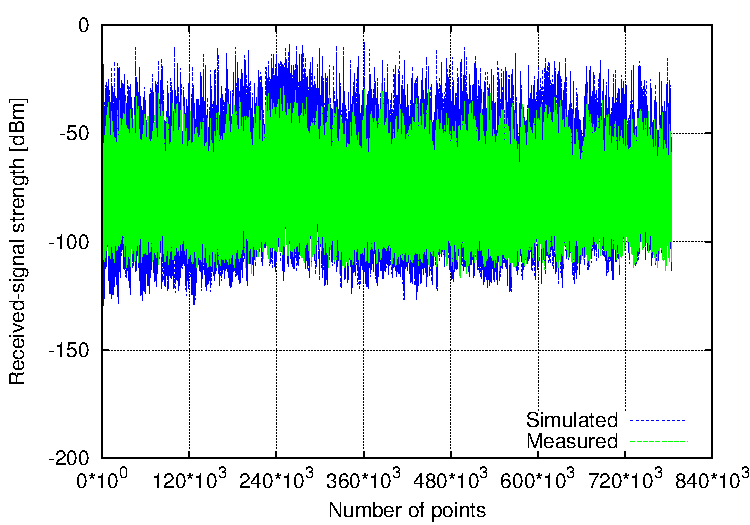
\includegraphics[width=0.47\textwidth]{08-real_network_planning/img/gsm_prato_rcv_pwr}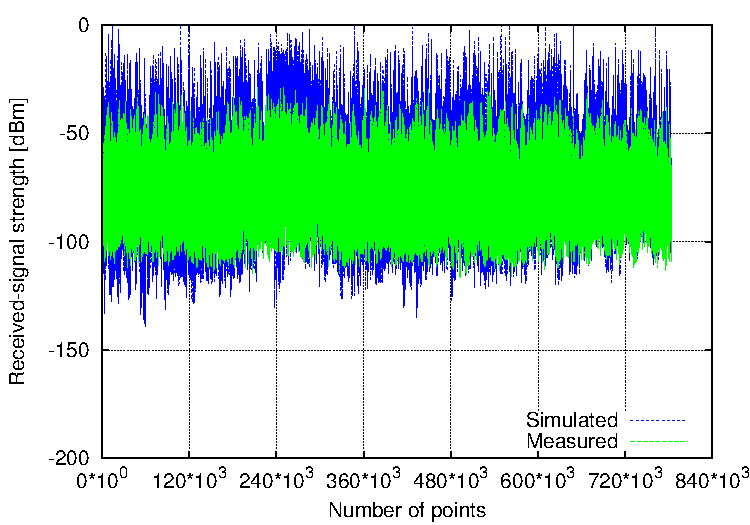
\includegraphics[width=0.47\textwidth]{08-real_network_planning/img/gsm_tcpu_rcv_pwr}\\\hspace{0.4cm}(a)\hspace{6.7cm}(b)

\caption{Net$_{11}$ distribution of the predicted received-signal powers (GSM)
compared to field measurements for: (a) PRATO, and (b) the commercial
radio-planning tool.\label{fig:08-Received_signal_power-GSM}}
\end{figure}


\begin{figure}[h]
\centering

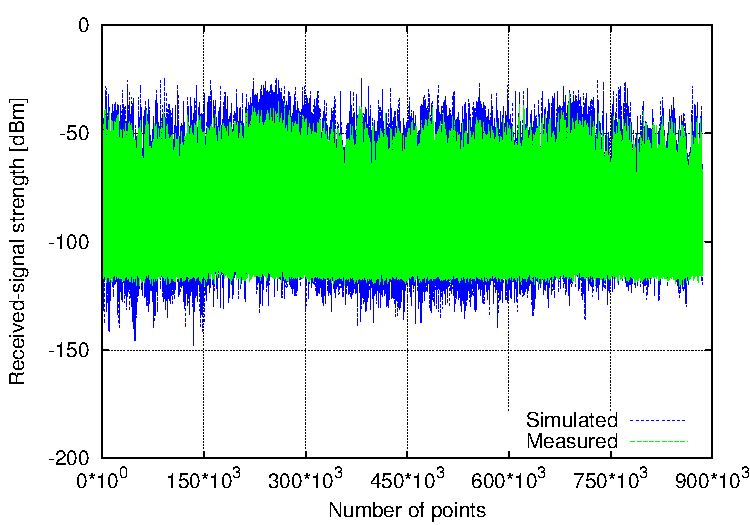
\includegraphics[width=0.47\textwidth]{08-real_network_planning/img/umts_prato_rcv_pwr}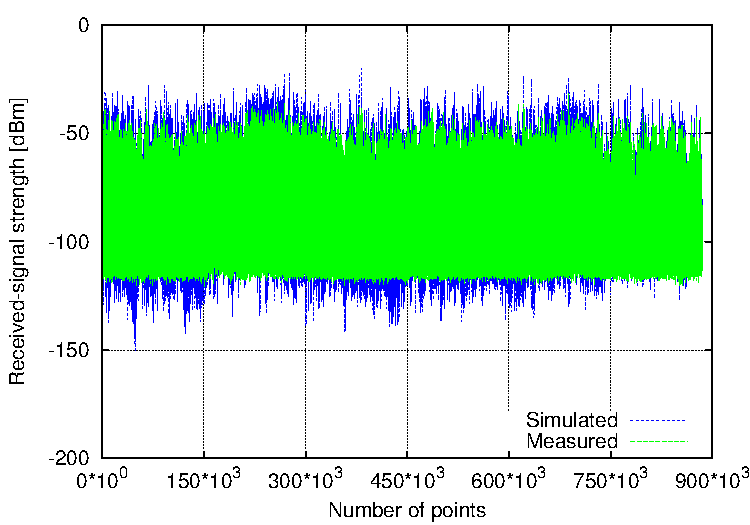
\includegraphics[width=0.47\textwidth]{08-real_network_planning/img/umts_tcpu_rcv_pwr}\\\hspace{0.4cm}(a)\hspace{6.7cm}(b)

\caption{Net$_{12}$ distribution of the predicted received-signal powers (UMTS)
compared to field measurements for: (a) PRATO, and (b) the commercial
radio-planning tool.\label{fig:08-Received_signal_power-UMTS}}
\end{figure}


\begin{figure}[H]
\centering

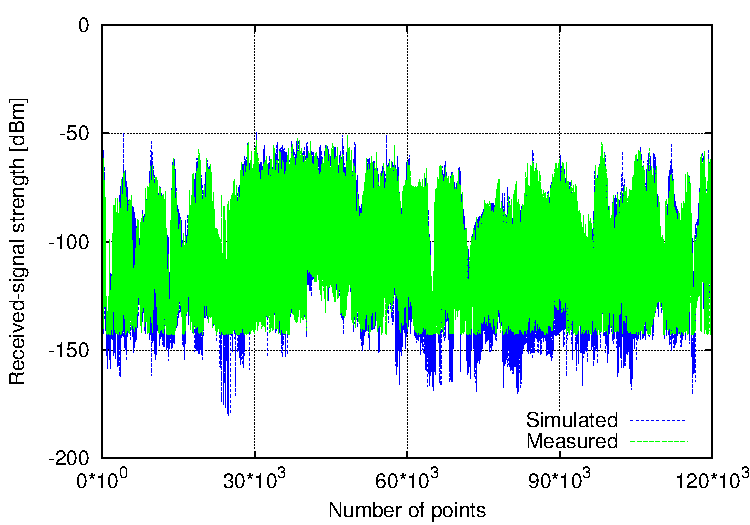
\includegraphics[width=0.47\textwidth]{08-real_network_planning/img/lte_prato_rcv_pwr}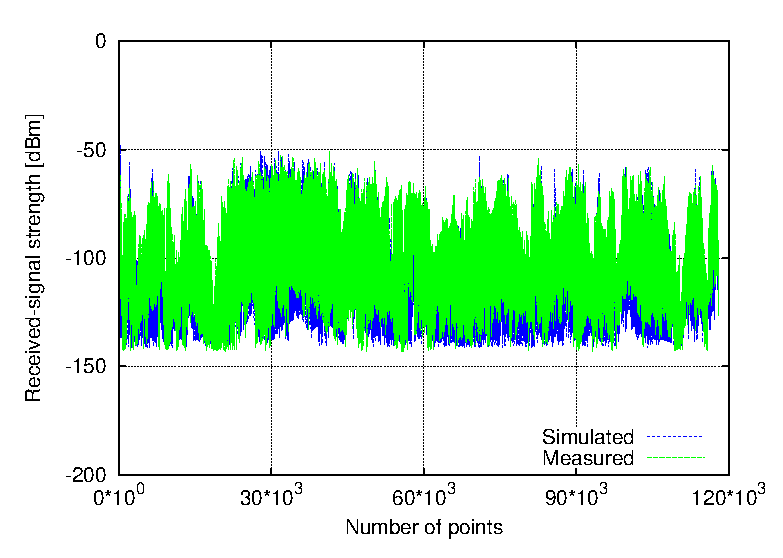
\includegraphics[width=0.47\textwidth]{08-real_network_planning/img/lte_tcpu_rcv_pwr}\\\hspace{0.4cm}(a)\hspace{6.7cm}(b)

\caption{Net$_{13}$ distribution of the predicted received-signal powers (LTE)
compared to field measurements for: (a) PRATO, and (b) the commercial
radio-planning tool.\label{fig:08-Received_signal_power-LTE}}
\end{figure}


Figure~\ref{fig:08-Received_signal_power-GSM}~(a), that depicts
the received-power levels for Net$_{11}$ (GSM), shows that the prediction
results match the field measurements rather well. A similar result
arrangement can be observed in Figure~\ref{fig:08-Received_signal_power-UMTS}~(a)
for Net$_{12}$ (UMTS), whereas the prediction results for Net$_{13}$
(LTE) show a slightly increased deviation from the field measurements,
as presented in Figure~\ref{fig:08-Received_signal_power-LTE}~(a).

\begin{figure}[h]
\centering

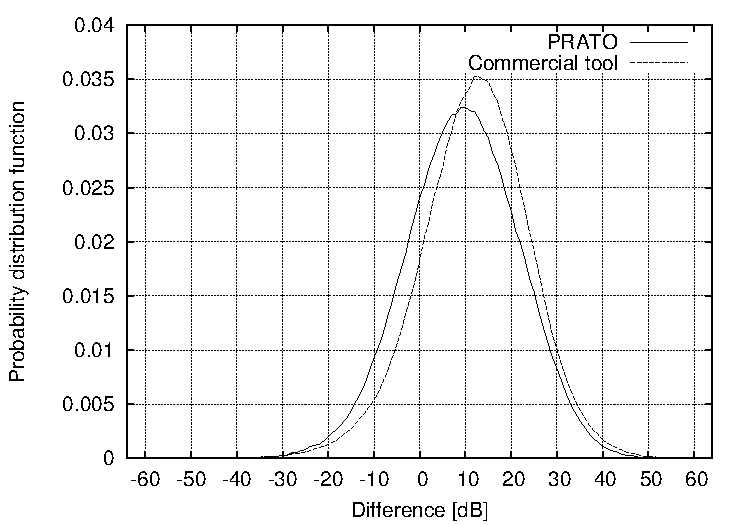
\includegraphics[width=0.6\textwidth]{08-real_network_planning/img/gsm_diff}

\caption{Probability distribution function for Net$_{11}$ (GSM) of the difference
between the field measurements and the simulation results of PRATO,
and the commercial tool. \label{fig:08-Prediction_difference-GSM}}
\end{figure}


\begin{figure}[h]
\centering

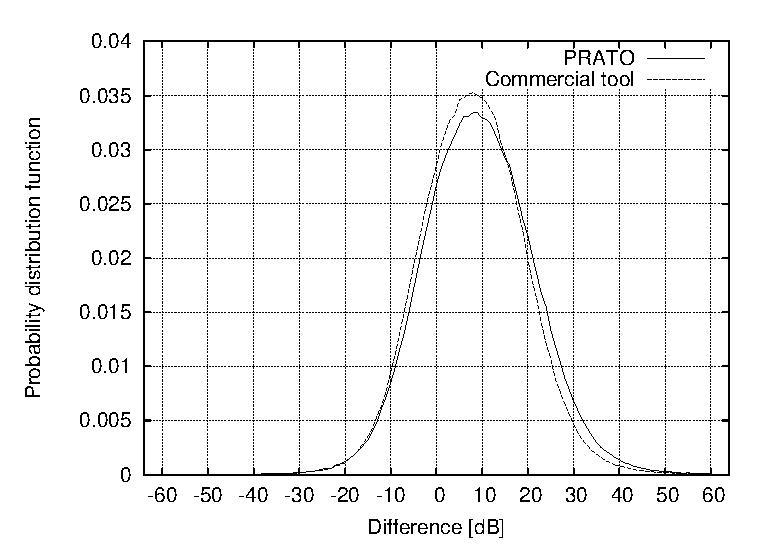
\includegraphics[width=0.6\textwidth]{08-real_network_planning/img/umts_diff}

\caption{Probability distribution function for Net$_{12}$ (UMTS) of the difference
between the field measurements and the simulation results of PRATO,
and the commercial tool.\label{fig:08-Prediction_difference-UMTS}}
\end{figure}


\begin{figure}[h]
\centering

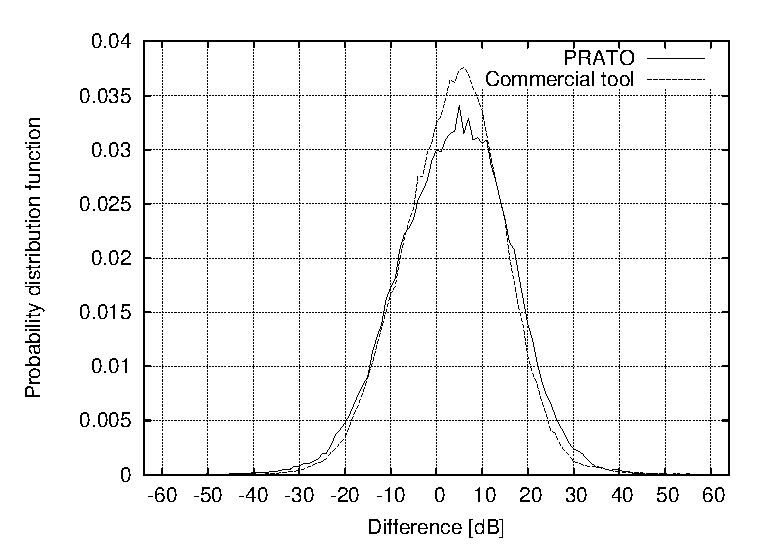
\includegraphics[width=0.6\textwidth]{08-real_network_planning/img/lte_diff}

\caption{Probability distribution function for Net$_{13}$ (LTE) of the difference
between the field measurements and the simulation results of PRATO,
and the commercial tool.\label{fig:08-Prediction_difference-LTE}}
\end{figure}


Plots showing the probability distribution function (PDF\nomenclature[A]{PDF}{Probability distribution function})
of the difference between the simulation results and the field measurements
were also produced. In this case, Figures~\ref{fig:08-Prediction_difference-GSM},
\ref{fig:08-Prediction_difference-UMTS}, and~\ref{fig:08-Prediction_difference-LTE}
show graphs representing the difference, expressed in dB, between
the predictions and measurements of Net$_{11}$, Net$_{12}$ and Net$_{13}$,
respectively. Again, the graphs labeled as (a) show the analysis for
PRATO, whereas the ones labeled as (b) show the same analysis for
the commercial tool. Table~\ref{tab:08-PDF_properties} lists the
mean and standard deviation of the PDFs for each network and tool
tested, the values of which are expressed in dB. It is important to
note that the parameter set used for both tools intentionally generate
pessimistic results in terms of coverage prediction. This is clearly
observed from the mean-difference values of all three test cases.

\begin{table}
\centering

\caption{Mean and standard-deviation values for the PDFs of the difference
between simulation and measurement results.\textit{\emph{ }}\textit{\label{tab:08-PDF_properties}}}


\begin{tabular}{cccccc}
\cmidrule{2-6} 
 & \multicolumn{2}{c}{Mean {[}dB{]}} &  & \multicolumn{2}{c}{Std. deviation {[}dB{]}}\tabularnewline\addlinespace
\cmidrule{2-6} 
 & PRATO & Commercial tool &  & PRATO & Commercial tool\tabularnewline\addlinespace
\midrule
Net$_{11}$ & 9.37 & 12.04 &  & 12.29 & 11.98\tabularnewline
Net$_{12}$ & 9.31 & 8.71 &  & 11.94 & 11.23\tabularnewline
Net$_{13}$ & 3.84 & 3.63 &  & 12.20 & 11.06\tabularnewline
\bottomrule
\end{tabular}
\end{table}


Comparing the plots for each of the test networks (see Figures~\ref{fig:08-Prediction_difference-GSM},
\ref{fig:08-Prediction_difference-UMTS}, and~\ref{fig:08-Prediction_difference-LTE}),
it is clear that the difference between each pair of (a) and (b) diagrams
is minor. A small difference is present on the commercial tool, the
predictions of which show a slightly greater deviation with respect
to the measurements. Therefore, it can be concluded that the prediction
results of PRATO are comparable with the results of the commercial
tool for the three test networks. Moreover, the presented analysis
also confirms that the calculated results are independent of the frequency
band used, since each test network operates in a different frequency.

Additionally, each of the test networks extended over different terrain
types and environments, e.g., urban and suburban areas. Since the
curves of the presented charts show similar profiles for the difference
between the measurements and simulations for both tools, the applicability
of PRATO for arbitrary terrain types can also be expected.

Notice also that PRATO generated similar results as the commercial
tool in all three cases, irrespective of the operational frequency
or chosen terrain type. The predicted values are also comparable for
different distances between the BSs and UEs. Moreover, a slight improvement
can be observed in some of the prediction values of PRATO, because
they better resemble the profile shown by the field measurements.


\subsection*{Computational-time performance}

In the following, the computational-time performance of both tools
is analyzed. The analysis focused on the required processing times
of both tools on the same system, the hardware of which consisted
of a 4-core Intel i7 2.67~GHz CPU, 24~GB of RAM and a dual nVidia
GeForce GTX 590 GPU. The simulations for PRATO were performed on a
Linux operating system, using multiple processes on the CPU. The commercial
tool required a Windows Server operating system, and provided single-process,
multi-threading support to use all the cores of the CPU.

The simulations included the test networks presented above, all of
which extend over a geographical region of 285~x~185~km$^{2}$,
with a resolution of 25~m. The processing times for a set of simulations
are given in Figures~\ref{fig:08-Running_times-GSM}, \ref{fig:08-Running_times-UMTS},
and~\ref{fig:08-Running_times-LTE}, for test networks Net$_{11}$,
Net$_{12}$ and Net$_{13}$, respectively.

\begin{figure}[h]
\centering

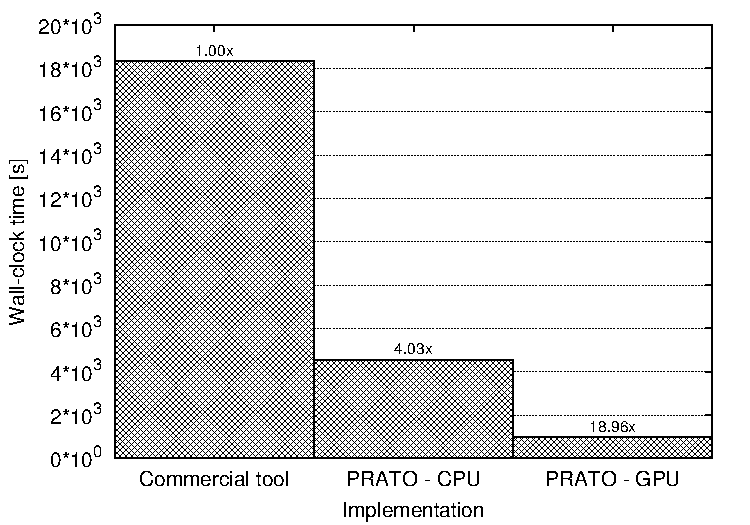
\includegraphics[width=0.7\textwidth]{08-real_network_planning/img/gsm_running_times}

\caption{Simulation-processing times and speedup factors of Net$_{11}$ (GSM)
for the commercial tool and two implementations of PRATO. \label{fig:08-Running_times-GSM}}
\end{figure}


\begin{figure}[h]
\centering

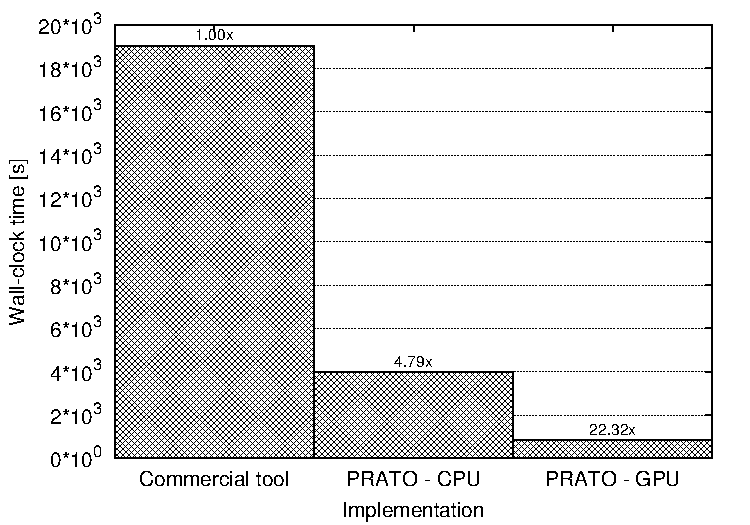
\includegraphics[width=0.7\textwidth]{08-real_network_planning/img/umts_running_times}

\caption{Simulation-processing times and speedup factors of Net$_{12}$ (UMTS)
for the commercial tool and two implementations of PRATO. \label{fig:08-Running_times-UMTS}}
\end{figure}


\begin{figure}[h]
\centering

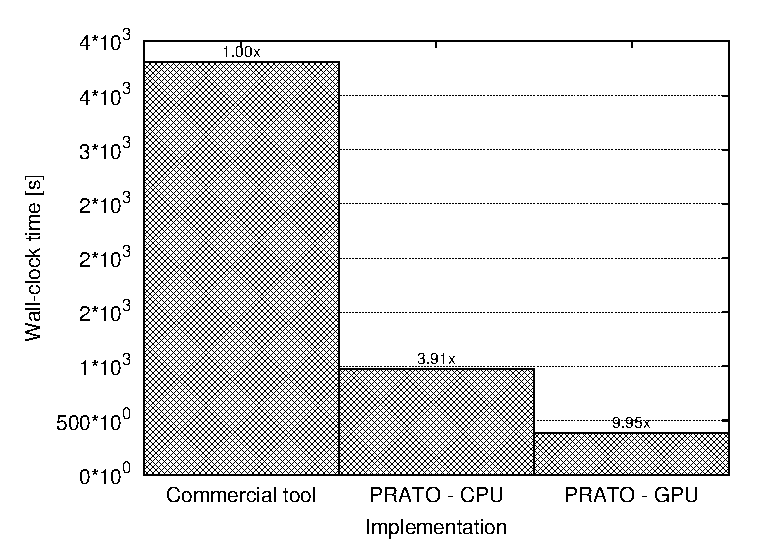
\includegraphics[width=0.7\textwidth]{08-real_network_planning/img/lte_running_times}

\caption{Simulation-processing times and speedup factors of Net$_{13}$ (LTE)
for the commercial tool and two implementations of PRATO. \label{fig:08-Running_times-LTE}}
\end{figure}


The plotted values represent the average simulation-processing time
after performing 10 independent measurements. The time-measurement
gathering was performed during the simulations presented in the previous
section. The PRATO-CPU deployed used six workers and one master process.
For the PRATO-GPU configuration, the same process deployment was used,
and the worker processes operated on the dual GPU, i.e., two GPUs
on one board, each of which featured 1.5~GB of DRAM. 

The benefits of the parallel implementation of PRATO is clear in all
three cases. Moreover, the multi-GPU support increases the running-time
performance even further, achieving speedup factors of 18.96, 22.32,
and 9.95, for Net$_{11}$, Net$_{12}$, and Net$_{13}$, respectively.
These results confirm that the use PRATO as a radio-planning tool
in a real-world environment is feasible and it outperforms the compared
commercial tool in terms of computational-time performance.


\section{Summary}

The radio planning of modern cellular networks requires efficient
and exact radio-signal coverage calculations. In this context, the
unified framework PRATO was evaluated from a radio-network planning
point-of-view by comparing its simulation results with field measurements.
The same analysis was applied to a professional software application
in order to assess the results of PRATO from a quality and performance
perspectives.

The extensive analyses presented in this chapter showed satisfactory
results. Compared to a professional network-planning tool, the result
accuracy achieved is completely comparable irrespective of the terrain
type or operational frequency, while the computational speed is many
times higher. These results confirm that PRATO does not reduce the
solution quality due to the increased performance. Indeed, its suitability
for use in a real-world environment, addressing different radio-planning
activities by simulation, was also confirmed. This fact makes the
framework interesting for researchers as well as for radio-network
engineers.
